% !TEX root = DesignDocument.tex



\section{Resumes}

%Your resumes are included here.  See the source file (industrial.tex) and uncomment the PDF includes to see how this works.  If your resume is written in \LaTeX\ then you can just insert the %\LaTeX\ source code.

Below are the resumes for the group members: Johnathon Ackerman, Daniel Andrus, Charles Bonn, Evan Hammer, and Joseph Mowry.


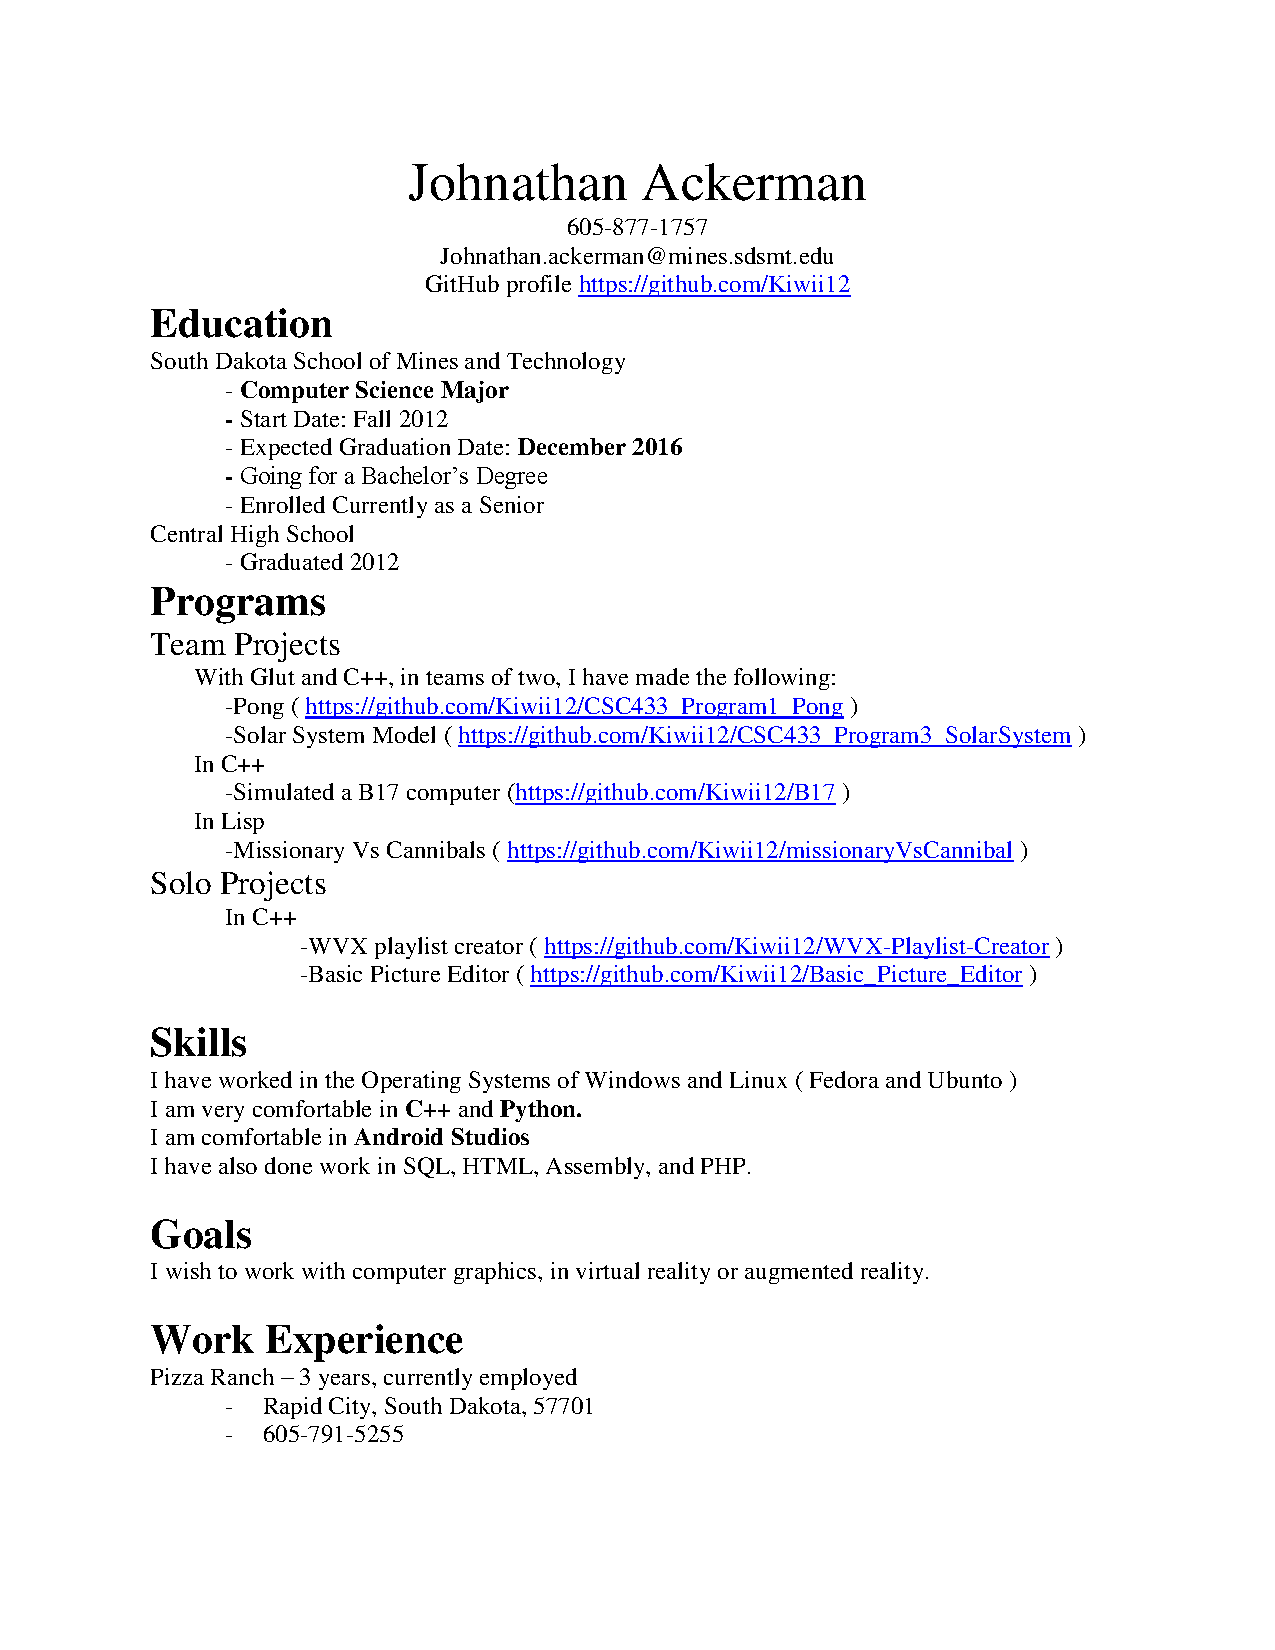
\includepdf{Additional/resumes/JohnathonAckermanResume.pdf}
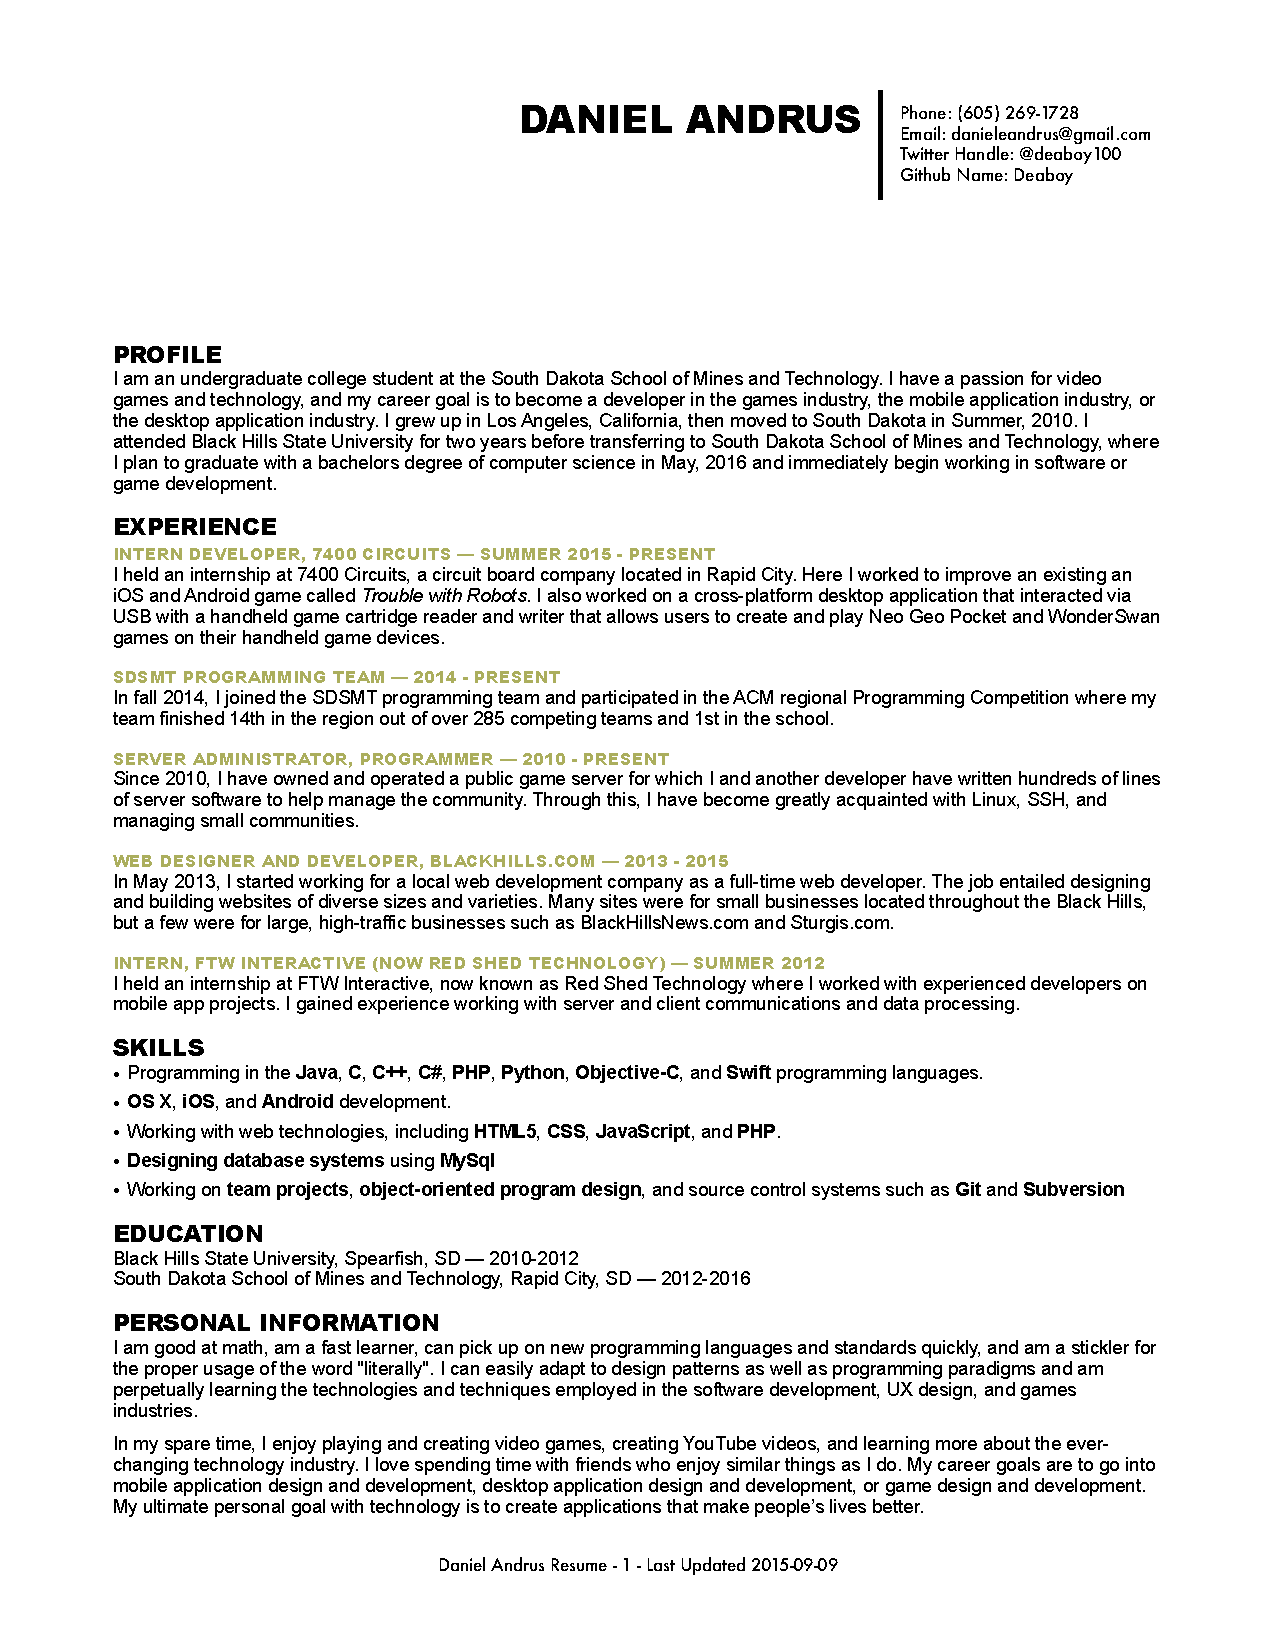
\includepdf{Additional/resumes/DanAndrusResume.pdf}
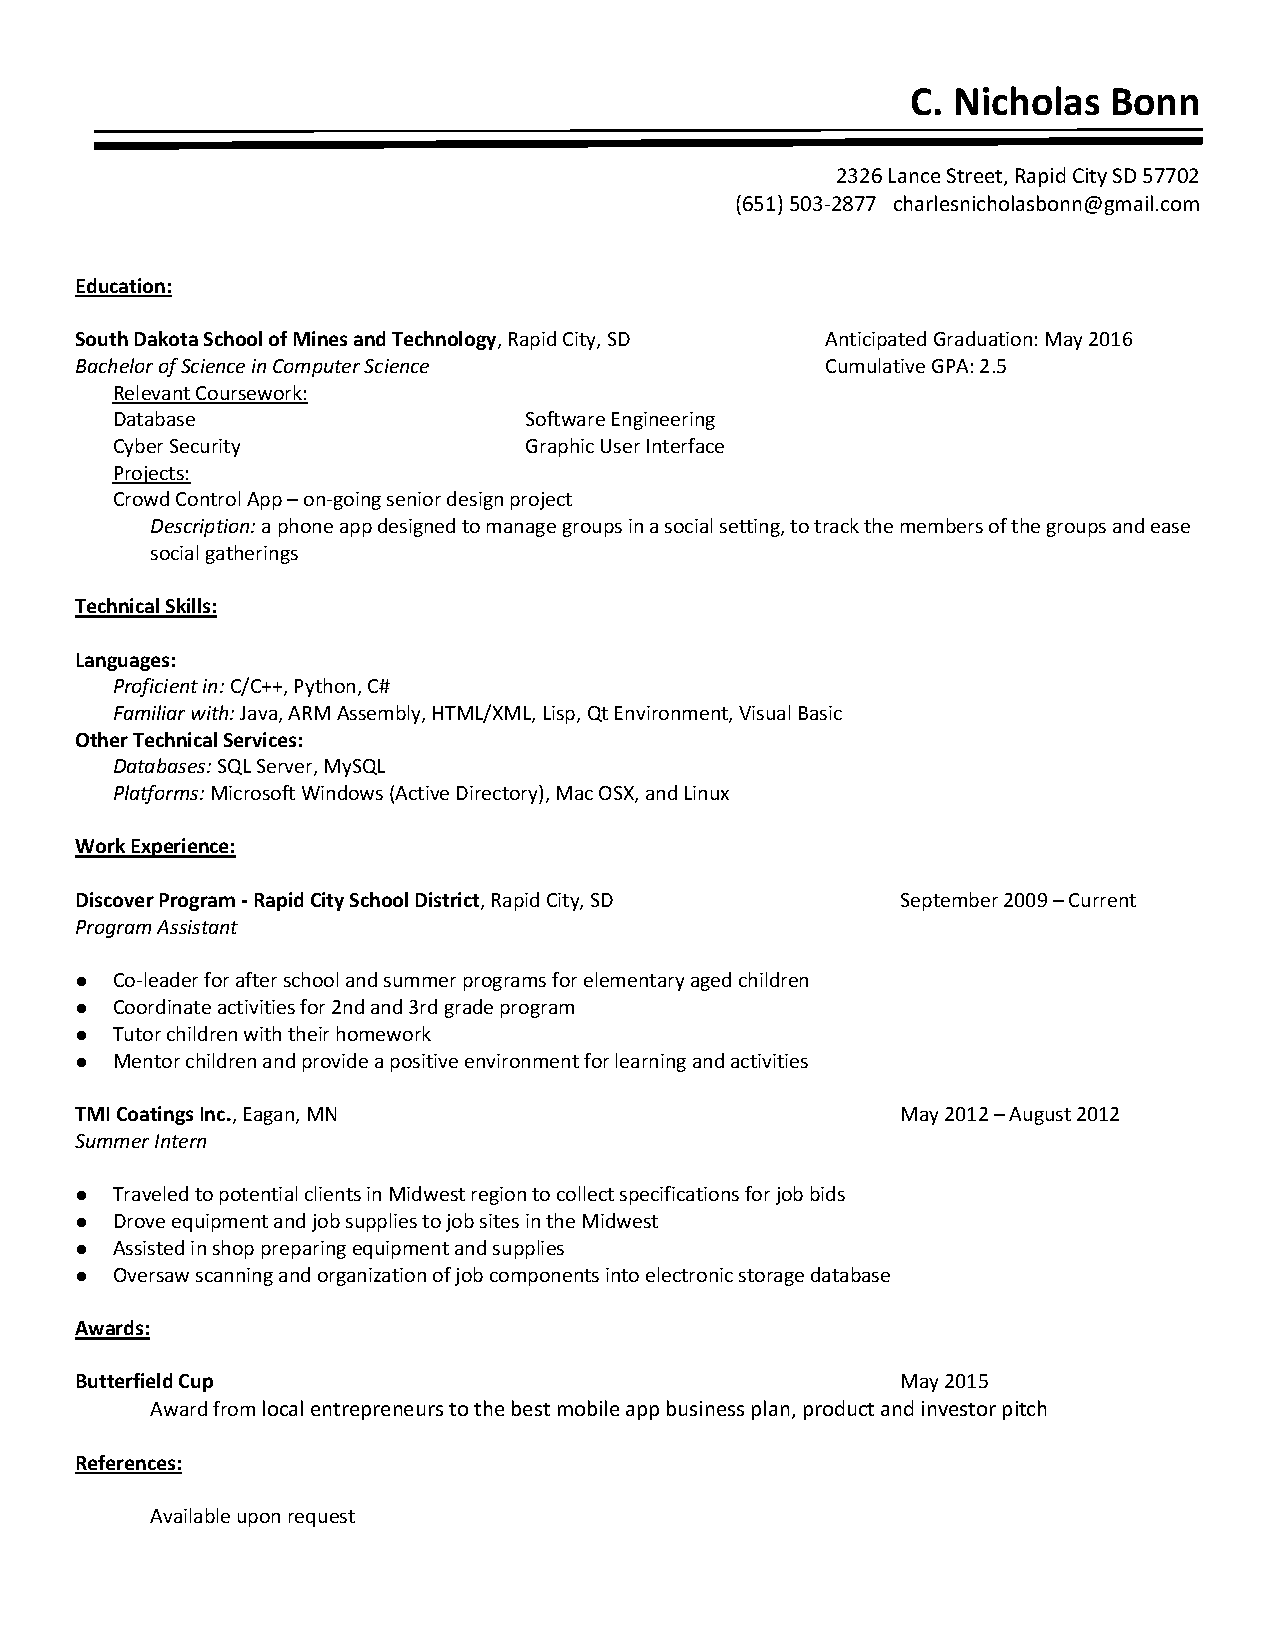
\includepdf{Additional/resumes/NickBonnResume.pdf}
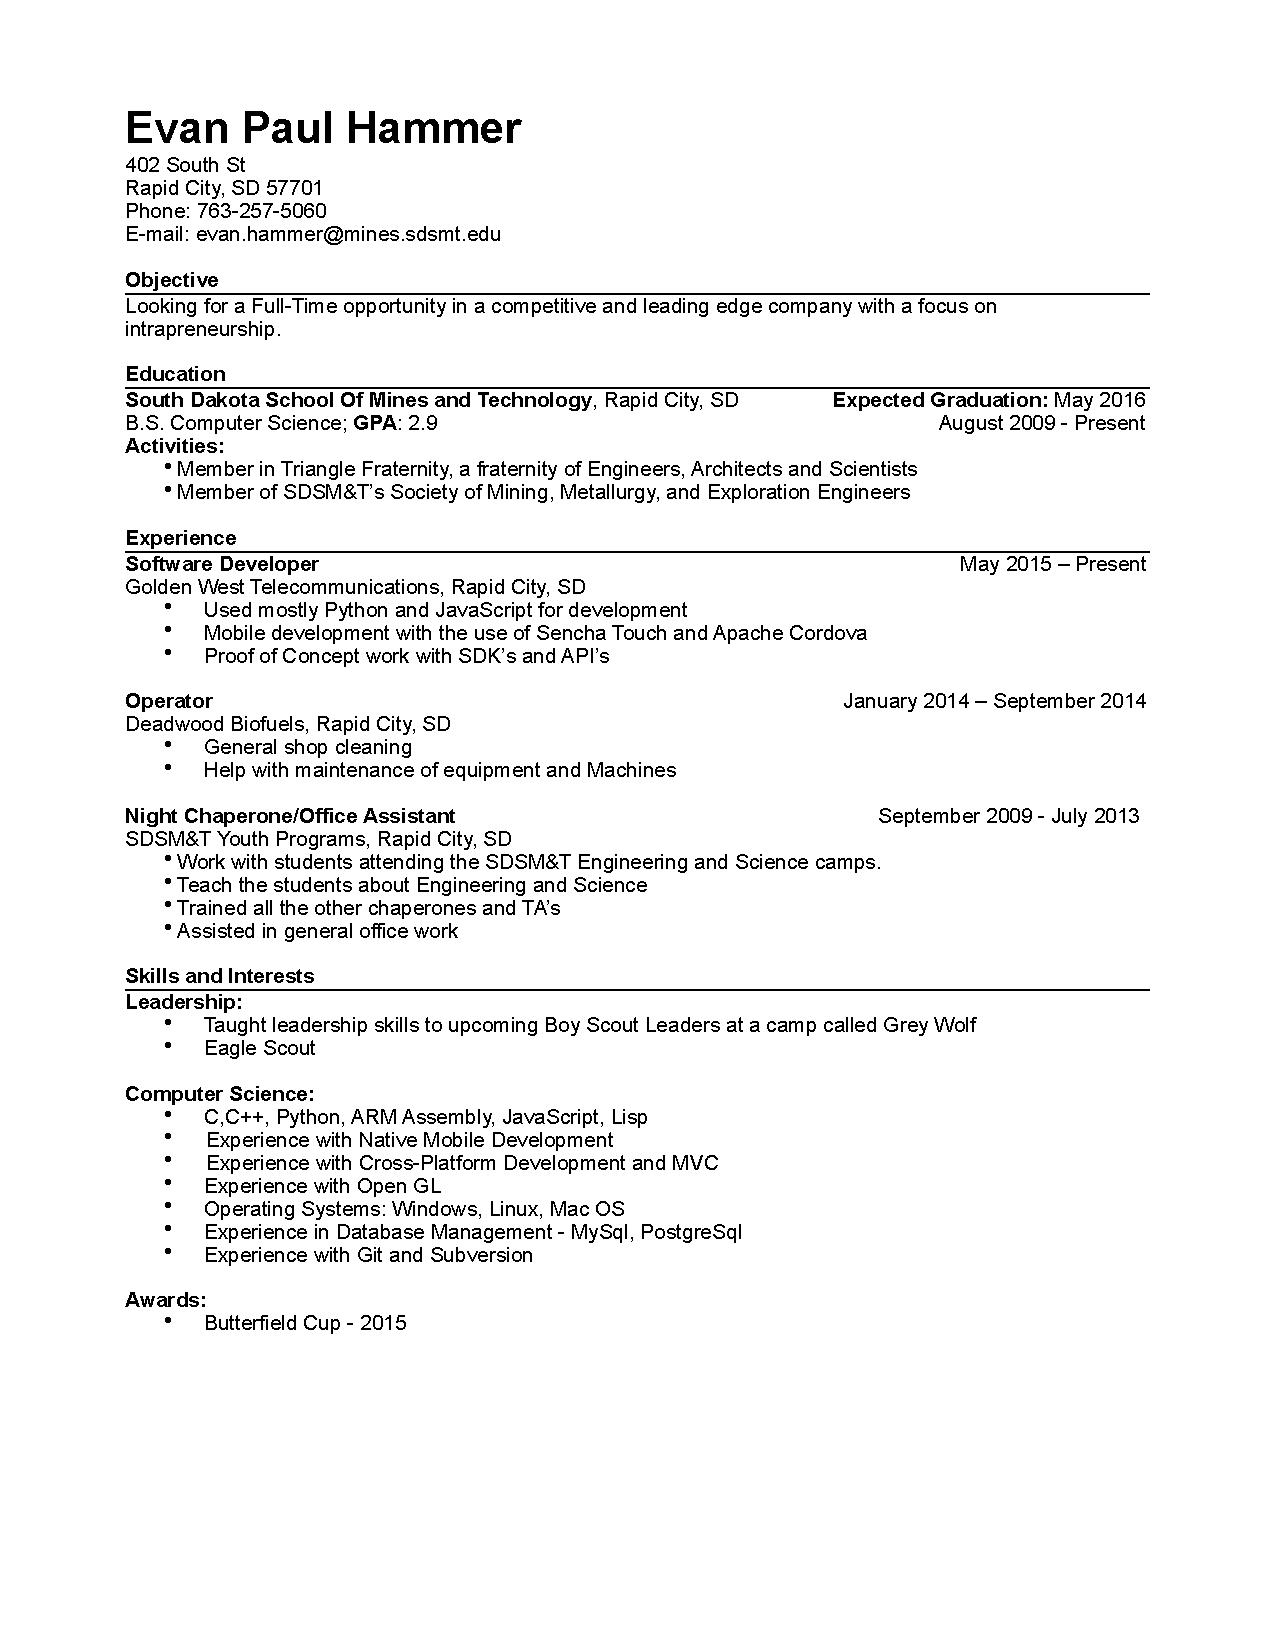
\includepdf{Additional/resumes/EvanHammerResume.pdf}
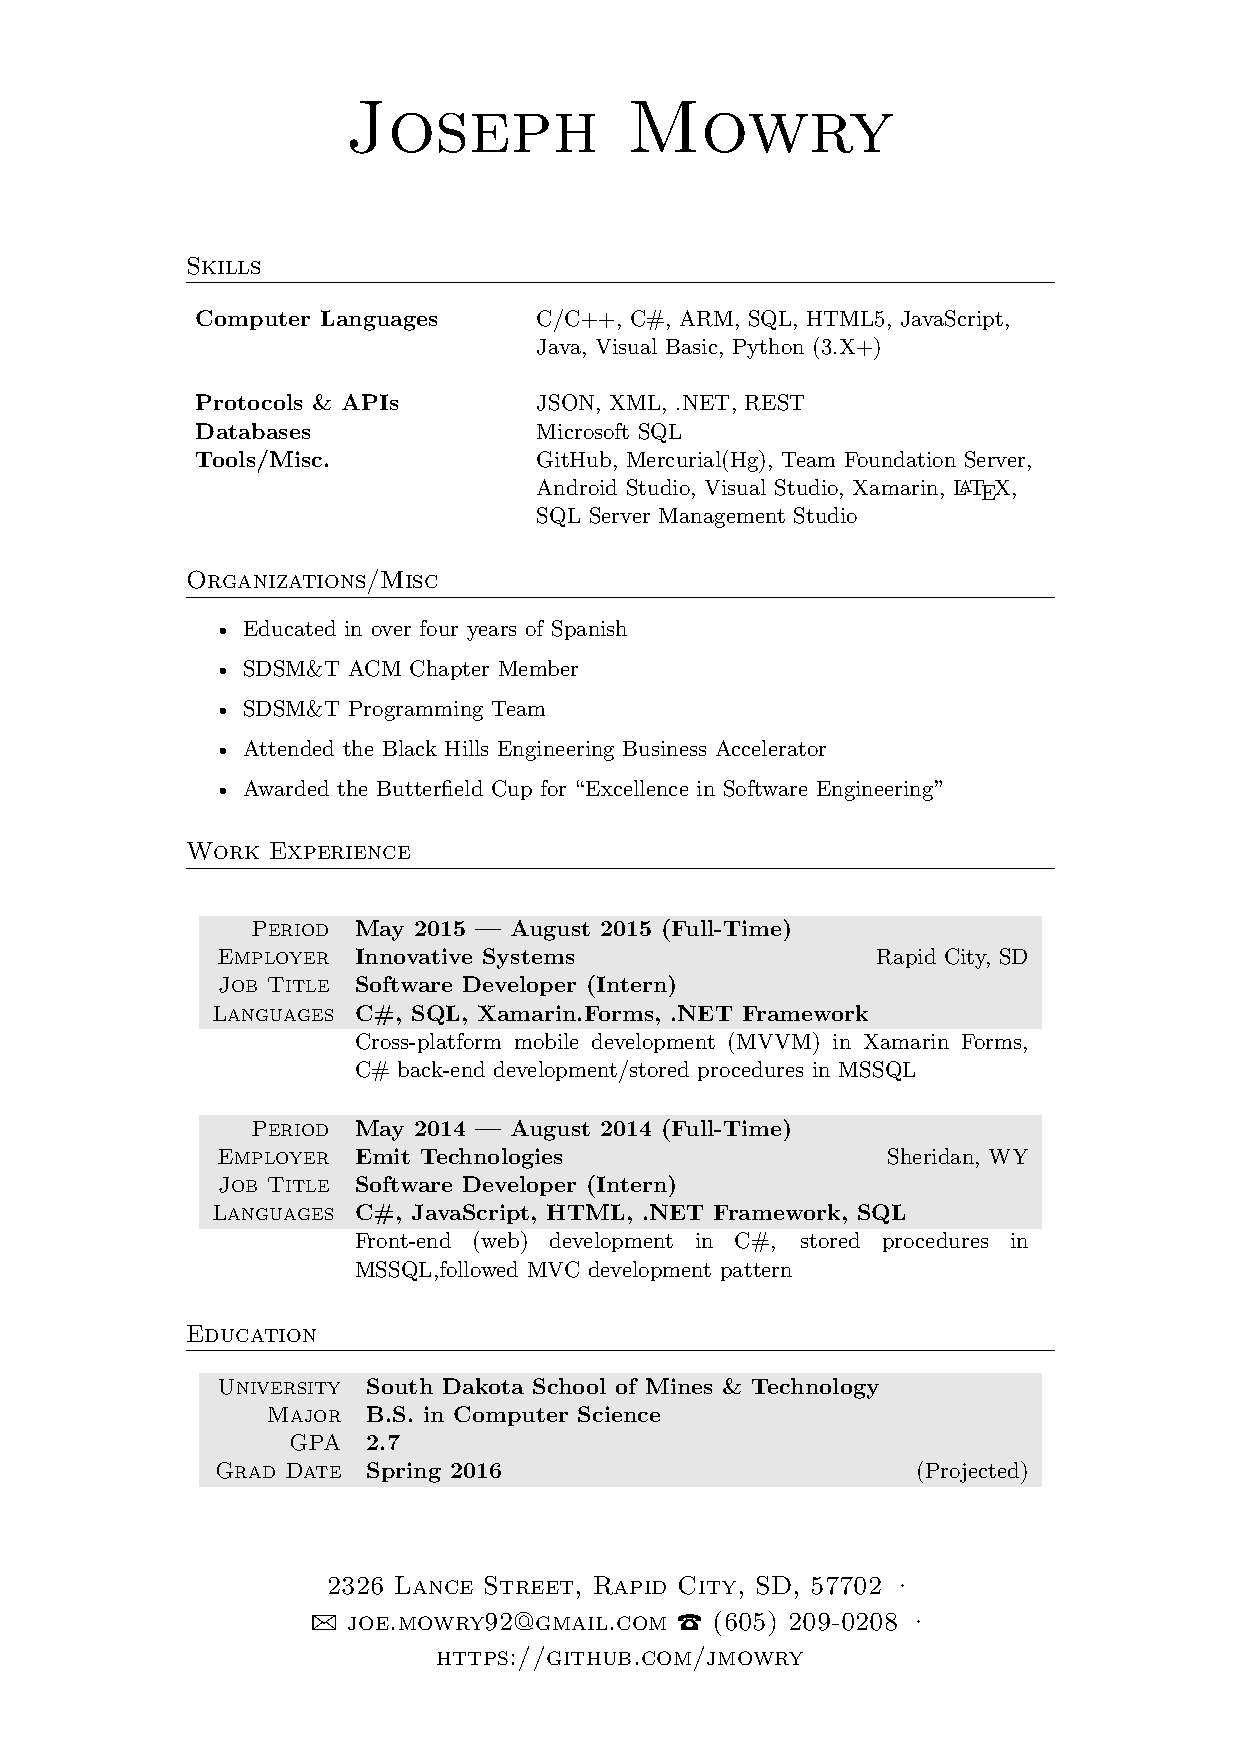
\includepdf{Additional/resumes/JosephMowryResume.pdf}

%    \includepdf[pages={1}]{report.pdf}  %% example of limited page include

%     \includepdf{resume1.pdf}
%     \includepdf{resume2.pdf}
%     \includepdf{resume3.pdf}

\section{ABET:  Industrial Experience Reports}

As a group we have attended the  SD Engineering Accelerator. We have compeated in multiple business plan competitions including:
	\begin{itemize}
	\item{Butterfield Cup}
	\item{SD Innovation Expo Business Plan Competition}
	\item{2015 SD Mines CEO Student Business Plan Competition}
	\end{itemize}
We also have also have and regular meetings with SDSMT EIR's to help format our buisness plan and Crowd Control.

\subsection{Johnathon Ackerman}

 I have had no Internship experience. However, before the project Crowd Control, I worked with C++, lisp, and python. I have worked with Visual Studios on Windows side, and Vim and G edit in Linux. 

\subsection{Daniel Andrus}

I first learned the basics of web design and development in high school. After my second year of college, I obtained an internship with FTW Interactive (now known as Red Shed Technologies). Later, I hold a position as Web Developer for 2 years before becoming an intern software developer at 7400 Circuits.

My course experience has ranged from data structures, image processing, database design, web development, group projects, computer graphics (including 3D graphics), mobile app development, and even compression.

\subsection{Charles Bonn}

I currently have little internship experence. What industry experence i do have is HTML. In my personal/professional life i help manage a website and a minecraft server. Though this is work i have worked with HTML and C code. I have also worked with game code that is java based.

\subsection{Evan Hammer}

I am working for Golden West Telecommunications(GW), a rural telecommunications provider in the state of South Dakota.  Since May of 2015 I have been a Software Developer for GW working on both mobile and back-end products.  For the mobile side, I have been working with a product called Cordova that is wrapped with another product called Sencha Touch.  Together these two products allow a developer to use JavaScript, HTML, CSS and more to produce a mobile application for Android, iOS and many other mobile platforms.  I have also written the back-end for this app, using Python and a PostgreSQL Database creating a server-side API for the mobile application.  While I am not working on the mobile application I have spent my time working on other in-house products using languages like Python and JavaScript.  These projects have ranged from updating existing code to ground-up projects.  Also as a Software Developer for GW, I have been tasked with creating some proof of concept work.  This work has ranged from testing possible new services as well as testing new platforms for development.  My work continues to grow and change as I continue to work for Golden West Telecommunications.

\subsection{Joseph Mowry}

In his pirior industry experience, Joseph specialized in C\# development and database management. His employers gave him a solid footing in AGILE and Scrum methodologies, as well as general product development. Though his experience lies primarily on the Visual Studio/C\# side of things, there is a large amount of skill overlap in Android Studio and Java that he can bring to the table for this project.





